\newpage
\section{Особенности вычислений на GPU}

\subsection{Преимущества перед решением на ЦП}

Задача интерактивной визуализации состоит не только в изображении, но и в просчете данных.
В случае с большим количеством оперативно взаимодействующих между собой объектов, вычисление
на графическом процессоре может значительно увеличить производительность за счет параллельности,
заложенной в архитектуру графической карты. В этом случае данные о каждой из частиц могут быть
представлены либо как вершинные, либо храниться в кадровых буферах.

Большая часть операций, выполняемых для просчета физики частиц работает с векторами. Графический
процессор позволяет оперировать векторами, имеет реализации стандартных операций
(сложение, вычитание, умножение, деление и т.п.). Кроме того предоставляет возможность вычислять
комплексные операции (например поиск отраженного вектора). Для центральных процессоров необходимо 
вручную писать реализацию векторных операций.

После обработки данных, информация о каждом объекте уже будет храниться в памяти графической карты.
Это значит что для визуализации достаточно вывести содержимое на экран.

В таблице \ref{tab:cpugpu} приведено сравнение вычислительных мощностей центральных и графических
процессоров \cite{gpu}.

\begin{table}[h!]
  \caption{\label{tab:cpugpu} Сравнение ЦП и ГП}
  \begin{center}
    \begin{tabular}{|c|l|c|c|c|}
      \hline
      Тип & Процессор & Кол-во ядер & АЛУ & Ширина SIMD \\
      \hline
      ГП & AMD Radeon HD 4870 & 10 & 80 & 64 \\
         & NVIDIA GeForce GTX 280 & 30 & 8 & 32 \\
      \hline
      ЦП & Intel Core 2 Quad & 4 & 8 & 4 \\
         & STI Cell BE & 8 & 4 & 4 \\
         & Sun UltraSPARC T2 & 8 & 1 & 1 \\
      \hline
    \end{tabular}
  \end{center}
\end{table}

\subsection{Графический конвейер}

Графический конвейер -- основной компонент компьютерной графики. Задача конвейера преобразовать
данные трехмерные объекты, источники света, виртуальную камеру и шейдерные преобразования в 
двумерное изображение.

Первые версии конвейеров работали с жесткой логикой (Fixed-Function Pipeline) \cite{raytracing02}.
Программисты не имели особого контроля над процедурой визуализации, потому что большинство
операций было встроено в аппаратное обеспечение и их невозможно было изменить программно.

Современные графические процессоры предоставляют так называемый программируемый графический
конвейер, который позволяет программистам писать специальные программы (шейдеры), которые
описывают поведение конвейера. При правильном использовании, шейдеры могут быть весьма эффективным
инструментом для создания различных эффектов. GPU состоят из сотен поточных процессоров и следуют
принципу параллельных вычислений SIMD (Single Instruction, Multiple Data) \cite{gpu}. Таким образом
параллелизм осуществляется на уровне данных, когда одна и та же операция выполняется
на множестве данных.

Сам конвейер состоит из следующих частей \cite{hgpuw}:

\begin{enumerate}
  \item Массивы данных из центрального процессора загружаются на графический в вершинный буфер
    (vertex buffer object).

  \item Проходят через вершинный шейдер (vertex shader), в котором подвергаются обработке 
    непосредственно сами элементы массива. Обычно на данном этапе идут преобразования 
    координат объектов для афинных преобразований и создания перспективы. Так же 
    могут быть преобразования цвета и координат текстур, но создание новых вершин 
    (элементов) не возможно.

  \item Следующий шаг это геометрический шейдер. Данный тип программ не поддерживается
    стандартом WebGL. Однако реализован в новых графических процессорах. В отличие 
    от вершинного, геометрический шейдер может обрабатывать одновременно целые примитивы 
    (отрезок, треугольник и т.д.). Кроме того, есть возможность генерировать примитивы 
    ``на лету'' не задействуя при этом центральный процессор.

  \item Затем полученные вершины попадают на сборку (clipping). На этом этапе образуются
    примитивы. Вершины, которые выходят из радиуса видимости, отбрасываются.

  \item Растеризация. Трехмерные примитивы преобразуются в двухмерные фигуры. Каждая фигура
    разбивается на фрагменты размером с пиксель.

  \item Фрагментный (или пиксельный) шейдер. На этом этапе задается цвет каждого из фрагментов.
    Самый простой фрагментный шейдер формирует один пиксель в виде цвета. Более сложные могут 
    выводить до нескольких цветов одновременно. Данные программы имеют информацию о положении 
    точки на экране, текстуре и других данных, передаваемых между шейдерами.

  \item Полученное изображение записывается в буфер кадра и выводится на экран (если необходимо).
\end{enumerate}

Данные шаги и передаваемые между ними данные изображены на рисунке \ref{fig:gpu_pipeline}.

\begin{figure}
\begin{center}
  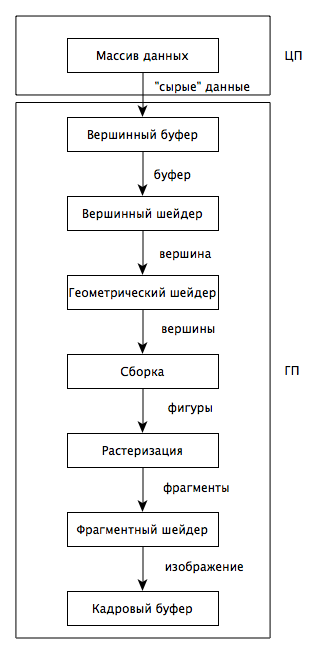
\includegraphics[scale=1.0]{Figures/gpu_pipeline}
\end{center}
\caption{Программируемый графический конвейер}
\label{fig:gpu_pipeline}
\end{figure}


\subsection{Язык шейдеров}

WebGL основан на стандарте OpenGL ES 2.0 \cite{khr11}, который поддерживает только программируемый графический
конвейер. Язык программирования, используемый для написания шейдеров, называется GLSL (OpenGL
Shading Language).

Поддерживаемые в данном стандарте типы шейдеров:

\begin{enumerate}
  \item Вершинные шейдеры. На входе: вершина фигуры. На выходе: преобразованное положение
    вершины. Результат вычислений записывается в специальную переменную gl\textunderscore{}Position.
  \item Фрагментные шейдеры. На входе: координаты на экране и данные, переданные из вершинного 
    шейдера. На выходе: цвет пикселя. Результат записывается в переменную gl\textunderscore{}FragColor.
\end{enumerate}

Когда вершинные и фрагментные шейдеры скомпилированы, они связываются в шейдерную программу.
В каждой программе может содержаться только один вершинный шейдер.

Доступность данных передаваемых внутри программ зависят от того, где они были инициализированы
и строго определяется какие операции могут на них выполнятся. В спецификации GLSL ES 1.0 
существует пять различных модификаторов типов:

\begin{itemize}
  \item локальные переменные (по умолчанию без ключевого слова);
  \item константы (ключевое слово const). Значения данного типа формируются во время компиляции и их не
    разрешено изменять при работе программы;
  \item аттрибуты (ключевое слово attribute). Загружаются на видеокарту из центрального процессора во время передачи массива данных. Видимы в 
    вершинных шейдерах. Значения данного типа также доступны в режиме только на чтение;
  \item одинаковые для всех шейдеров (ключевое слово uniform). Передаются с ЦП во время 
    использования программы. Доступны как в вершинных, так и в фрагментных;
  \item последний модификатор формирует связь между вершинным и фрагментным шейдером. Первый
    формирует какое-то значение для каждой вершины и передает его в вершинную программу.
    Ключевое слово varying.
\end{itemize}

Связи между модификаторами переменных и типами шейдеров изображены на рисунке \ref{fig:glsl_vars}.

\begin{figure}
\begin{center}
  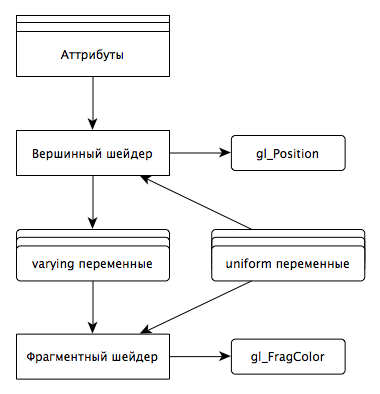
\includegraphics[scale=1]{Figures/glsl_vars}
\end{center}
\caption{Связи между модификаторами переменных и типами шейдеров в GLSL}
\label{fig:glsl_vars}
\end{figure}


\subsection{Кадровые буферы}

Кадровым буфером называется область памяти для кратковременного хранения данных перед отправкой
на устройство вывода. Данный буфер содержит полную информацию о цветах (значениях) кадра.

Значения кадрового буфера формируется на выходе фрагментного шейдера. Это значит что их можно 
использовать как промежуточное хранилище данных при выполнении алгоритмов. Этап формирования 
конечного изображения через множество программ называются проходом (pass). Содержимое буферов 
можно считывать по известным координатам. Получаемые данные носят название тексел (текстурный 
пиксел). В данном подходе данные остаются непосредственно на видеокарте. Уходит необходимость
постоянно передавать данные на ЦП и обратно, что значительно увеличивает производительность.

Тип данных кадровых буферов определяется стандартом. Выход фрагментных шейдеров представлен в 
GLSL как четырехмерный вектор типа float (числа с плавающей точкой). Передача в другую программу
осуществляется через текстурные блоки. В спецификации WebGL по-умолчанию при связке текстуры
и кадрого буфера доступен только формат byte (неотрицательное число от 0 до 255) \cite{khr11}. 
Это значит что при вычислениях могут быть значительные потери при дискретизации данных. При помощи
расширения OES\textunderscore{}texture\textunderscore{}float можно включить поддержку передачи 
данных типа float.
